% The file name pays homage to White's Viscous Fluid Flow great section title:
% 3-8.1.2 Harbingers of boundary-layer behavior

\section{Stagnation flow}

In order to provide a glimse into the difficulties that are
encountered as soon as one ventures into slightly more complicated
problems, let us work out a solution of Navier-Stokes equations for a
simple stagnation situation.

The potential flow solution for a stady-state incompressible 2D
stagnation flow pattern close to a flat wall is given by the stream
function
\[
\psi = B x y ,
\]
from which,
\[
\begin{cases}
  & u_x =  \frac{\partial \psi}{\partial y} =   B x \\
  & u_y = -\frac{\partial \psi}{\partial x} = - B y .
\end{cases}
\]

The parameter $B$ has units of inverse time, and is given in practical
situations by $u_0 / L$, where $u_0$ is a relevant upstream velocity,
and $L$ a relevant size.

Recalling what we learned about potential flow and its relationship
with complex analysis, since $\psi = (B/2) \Im (z^2)$, it is easy to guess the
correct potential: $\phi=\Re( z^2) = (B/2) (x^2 + y^2)$.

This flow pattern looks roughly correct, see
Fig. \ref{fig:stagnation_streamlines} left, where the streamlines are
shown, along with the pressure. The latter follows from Bernoulli
principle:
\begin{equation}
  \label{eq:p_stag_pot}
p =
 -\frac{1}{2} \left[
  u_x ^2 +
  u_y^2
  \right] =
-\frac{1}{2} \left[
  (B x)^2 +
  (-B y)^2
  \right].  
\end{equation}


\begin{figure}
  \centering
  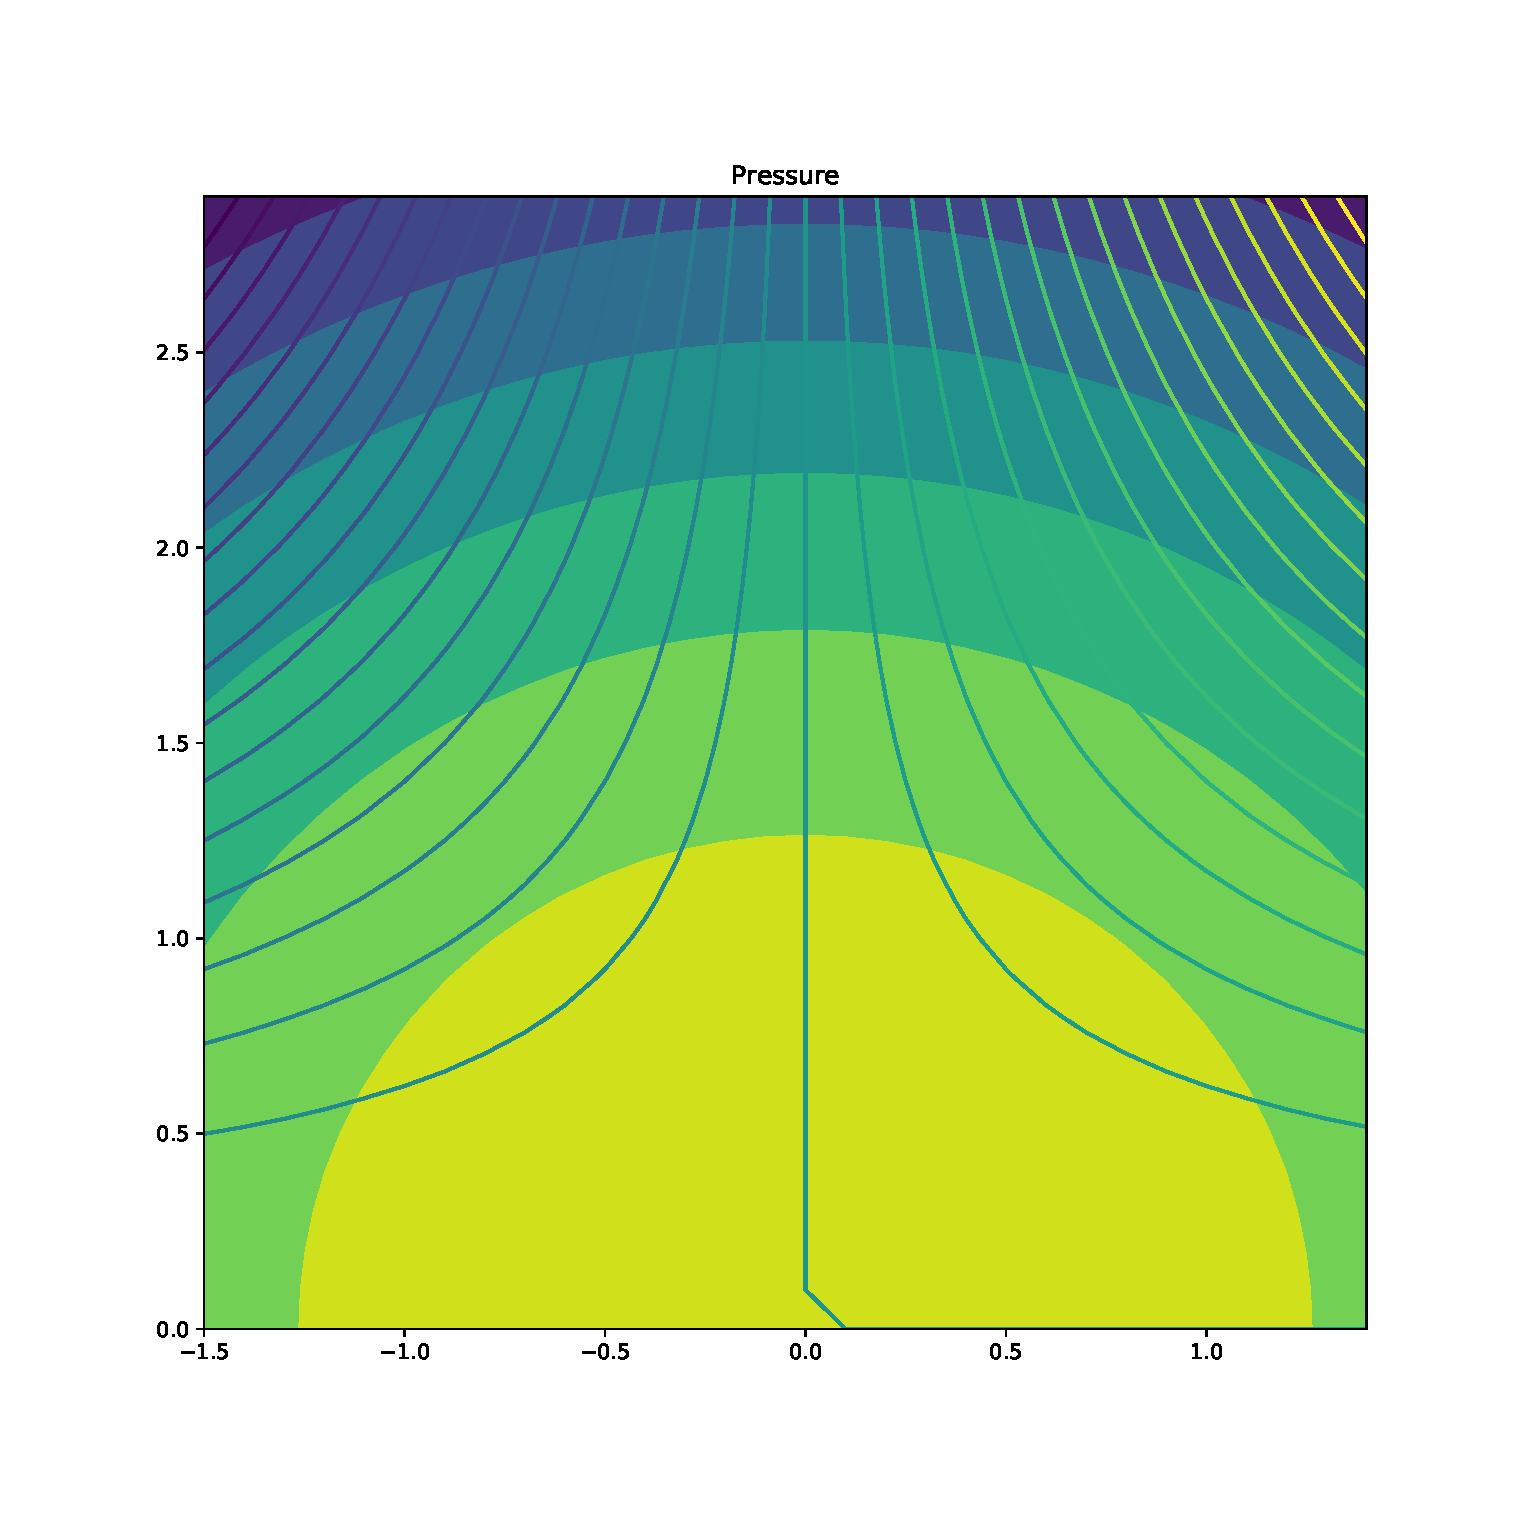
\includegraphics[width=0.4\linewidth]{figures/stagnation_potential_streamlines}
  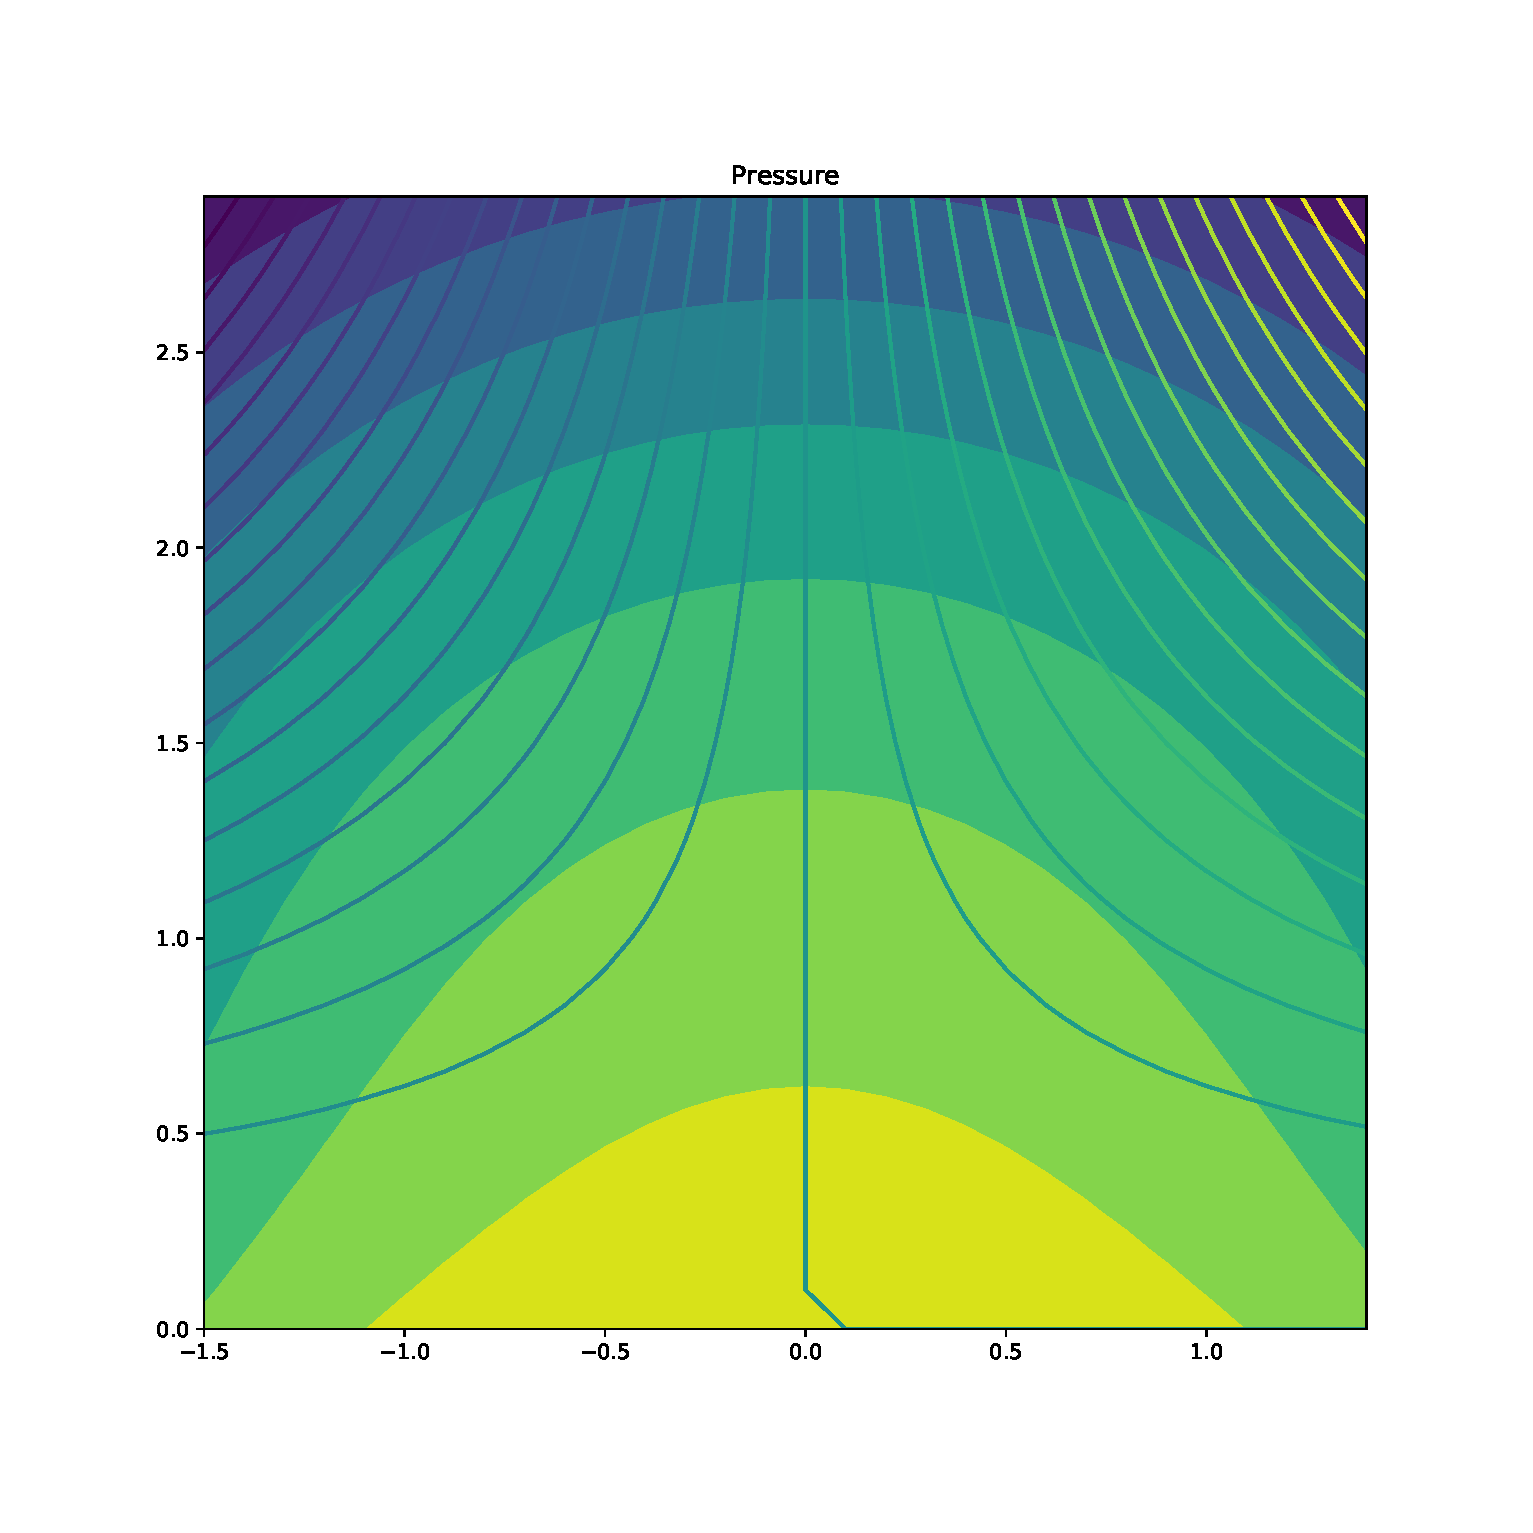
\includegraphics[width=0.4\linewidth]{figures/stagnation_viscous_streamlines}
  \caption{\label{fig:stagnation_streamlines}}
\end{figure}

But of course, at the wall ($y=0$) the fluid flows freely along the
wall. This means the boundary conditions are of the ``slip'' kind,
instead of the more realistic ``no-slip'' kind.

In order to find a correct flow, let us us the ansatz, originally
investigated by Hiemenz in 1911\footnote{%
  Hiemenz was a student of Prandtl, the founder of the theory of
  viscous boundary layers.
}.
  \[
\psi = B x f(y) ,
\]
where $f$ is a function of $y$ only. This is basically a separation of
variables, also guessing a linear dependence on $x$.

The velocity is now,
\[
\begin{cases}
  & u_x =   B x f' \\
  & u_y = - B f .
\end{cases}
\]
The correct no-slip condition then implies $f(0)=f'(0)=0$. We will
also require $f'(\infty)\to 1$ in order to recover our previous,
potential flow, solution.

Now, the steady 2D Navier-Stokes equations read
\begin{align}
  u_x  \frac{\partial u_x}{\partial x} +
  u_y  \frac{\partial u_x}{\partial y} 
  & =   - \frac{\partial p}{\partial x} +
  \nu
  \left(
  \frac{\partial^2 u_x}{\partial x^2} +
  \frac{\partial^2 u_x}{\partial y^2}
  \right) \\
  u_x  \frac{\partial u_y}{\partial x} +
  u_y  \frac{\partial u_y}{\partial y} 
  & =   - \frac{\partial p}{\partial y} +
  \nu
  \left(
  \frac{\partial^2 u_y}{\partial x^2} +
  \frac{\partial^2 u_y}{\partial y^2}
  \right) .
\end{align}
(Here, $p$ is not the true pressure, but the ``kinematic pressure'',
$p/\rho$. For convenience, a $\rho$ factor is assimilated into it, in
the same way that $\nu=\mu/\rho$.)

The $x$ equation is then reduced to
\[
 (B x f') (B f') + (-B f) B x f'' =  - \frac{\partial p}{\partial x} +
\nu B x f''' ,
\]
which may be written as
\[
B f f'' - B (f')^2 + \nu f''' = \frac{1}{B x} \frac{\partial
  p}{\partial x}  .
\]
Now, the left part of the equation is a function of $y$ only. This
means the pressure can only have this form:
\[
p(x,y) = C x^2 + h(y) ,
\]
with a constant $C$ and a function of $h$ to be determined later. Moreover,
as $y$ gets large we want to recover the potential solution. In this limit,
\[
f \to a + y \qquad f' \to 1 \qquad f'' \to 0 \qquad f'''\to 0 ,
\]
so the equation in this limit is
\[
- B \to  \frac{2 C x }{B x} ,
\]
which means $C =-B/2$, to be used later when solving for the pressure.

We must then solve
\[
 B \left(  f f'' + 1-  (f')^2 \right) + \nu f''' = 0 .
\]

Now, a lot may be learned from the shape of an equation without even
solving it. Let us look for a similarity transformation of the
form
\[
f(y) = b g(a y) ,
\]
so that equation for $f$ may be cast as an equation for $g$ with no
parameters. With this prescription,
\[
f' = ba g' \qquad f''=b a^2 g'' \qquad f'''= b a^3 g''' ,
\]
So then the equation reads
\[
 B \left(  b^2 a^2 g g'' + 1-  b^2 a^2 (g')^2 \right) + \nu b a^3  g''' = 0 .
\]
Because of the ``$1$'' in the parenthesis, it is clear $b=1/a$, so then,
\[
 B \left(  g g'' + 1-  (g')^2 \right) + \nu  a^2  g''' = 0 .
\]
Therefore, if $a=\sqrt{B/\nu}$,
\begin{equation}
  \label{eq:Z_ode}
  g g'' + 1-  (g')^2  +  g''' = 0 ,
\end{equation}
with no parameters, as we wanted. This means that, whichever solution
we find, our $f$ is going to be given by
\[
f(y) = \sqrt{\frac{\nu}{B}} g\left(\sqrt{\frac{B}{\nu}}  y  \right) =
\sqrt{\frac{\nu}{B}} g\left(\frac{y}{ \sqrt{\nu/B} } \right) =
 \ell g\left(\frac{y}{ \ell } \right) .
\]
Clearly, $\ell = \sqrt{\nu/B} $ sets the scale of variation of the
flow away from its potential solution.

Notice that the velocities will be
\[
\begin{cases}
  & u_x =   B x g'(y/\ell) = B\ell \frac{x}{\ell} g'(y/\ell)  \\
  & u_y = - B \ell g(y/\ell)  ,
\end{cases}
\]
so that the velocity scale is set by $B\ell=\sqrt{B\nu}$.


%The $y$ equation reduces, with our velocities, to
%\[
%B^2 f f' = - \frac{\partial p}{\partial y} - B\nu f'' .
%\]
%This means that $\frac{\partial p}{\partial y}$ is a function of $y$
%only.



Our task is then to integrate the non-linear ODE \ref{eq:Z_ode}, subject
to these boundary conditions:
\[
g(0)=0 \qquad g'(0)=0 \qquad g''(x\to \infty) \to 0 .
\]
If we had a condition on $g''(0)$, the problem would be a
straight-forward exercise in integration. However, we have instead a
condition on the other side of the integration domain, which makes
this problem somewhat harder. The technique should then be a
``shooting method'', in which $g''(0)$ is adjusted until a vanishing
small of $g''$ far away is found. The procedure may be made
systematic, but we can also fiddle a bit with the parameters in order
to find a reasoable approach. It is quite easy to arrive at
$g''(0)\approx 1.234$, as in the jupyter python notebook at
Supplementary Material.

%How far is far away may be again estimated from the equation.


\begin{figure}
  \centering
  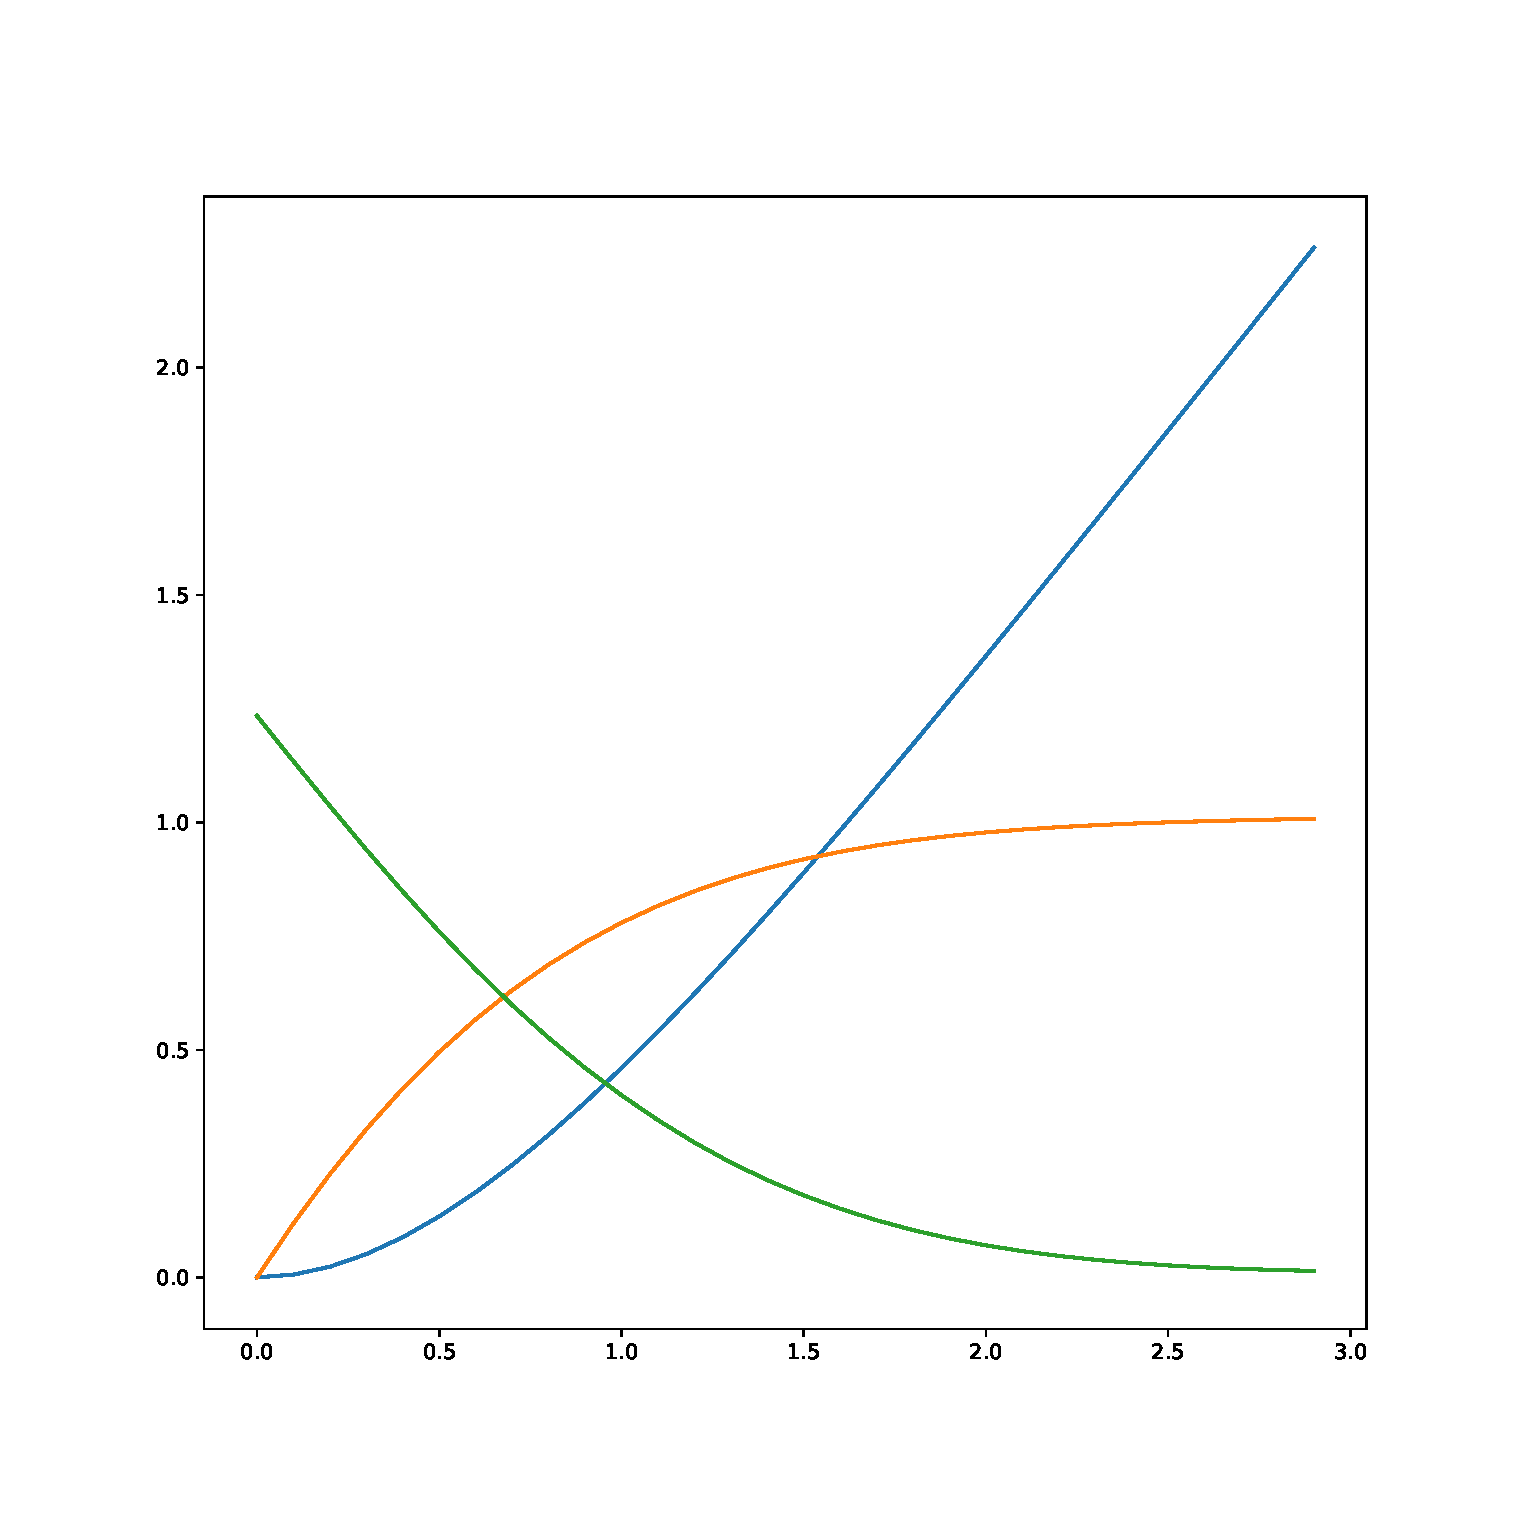
\includegraphics[width=0.4\linewidth]{figures/stagnation_functions}
    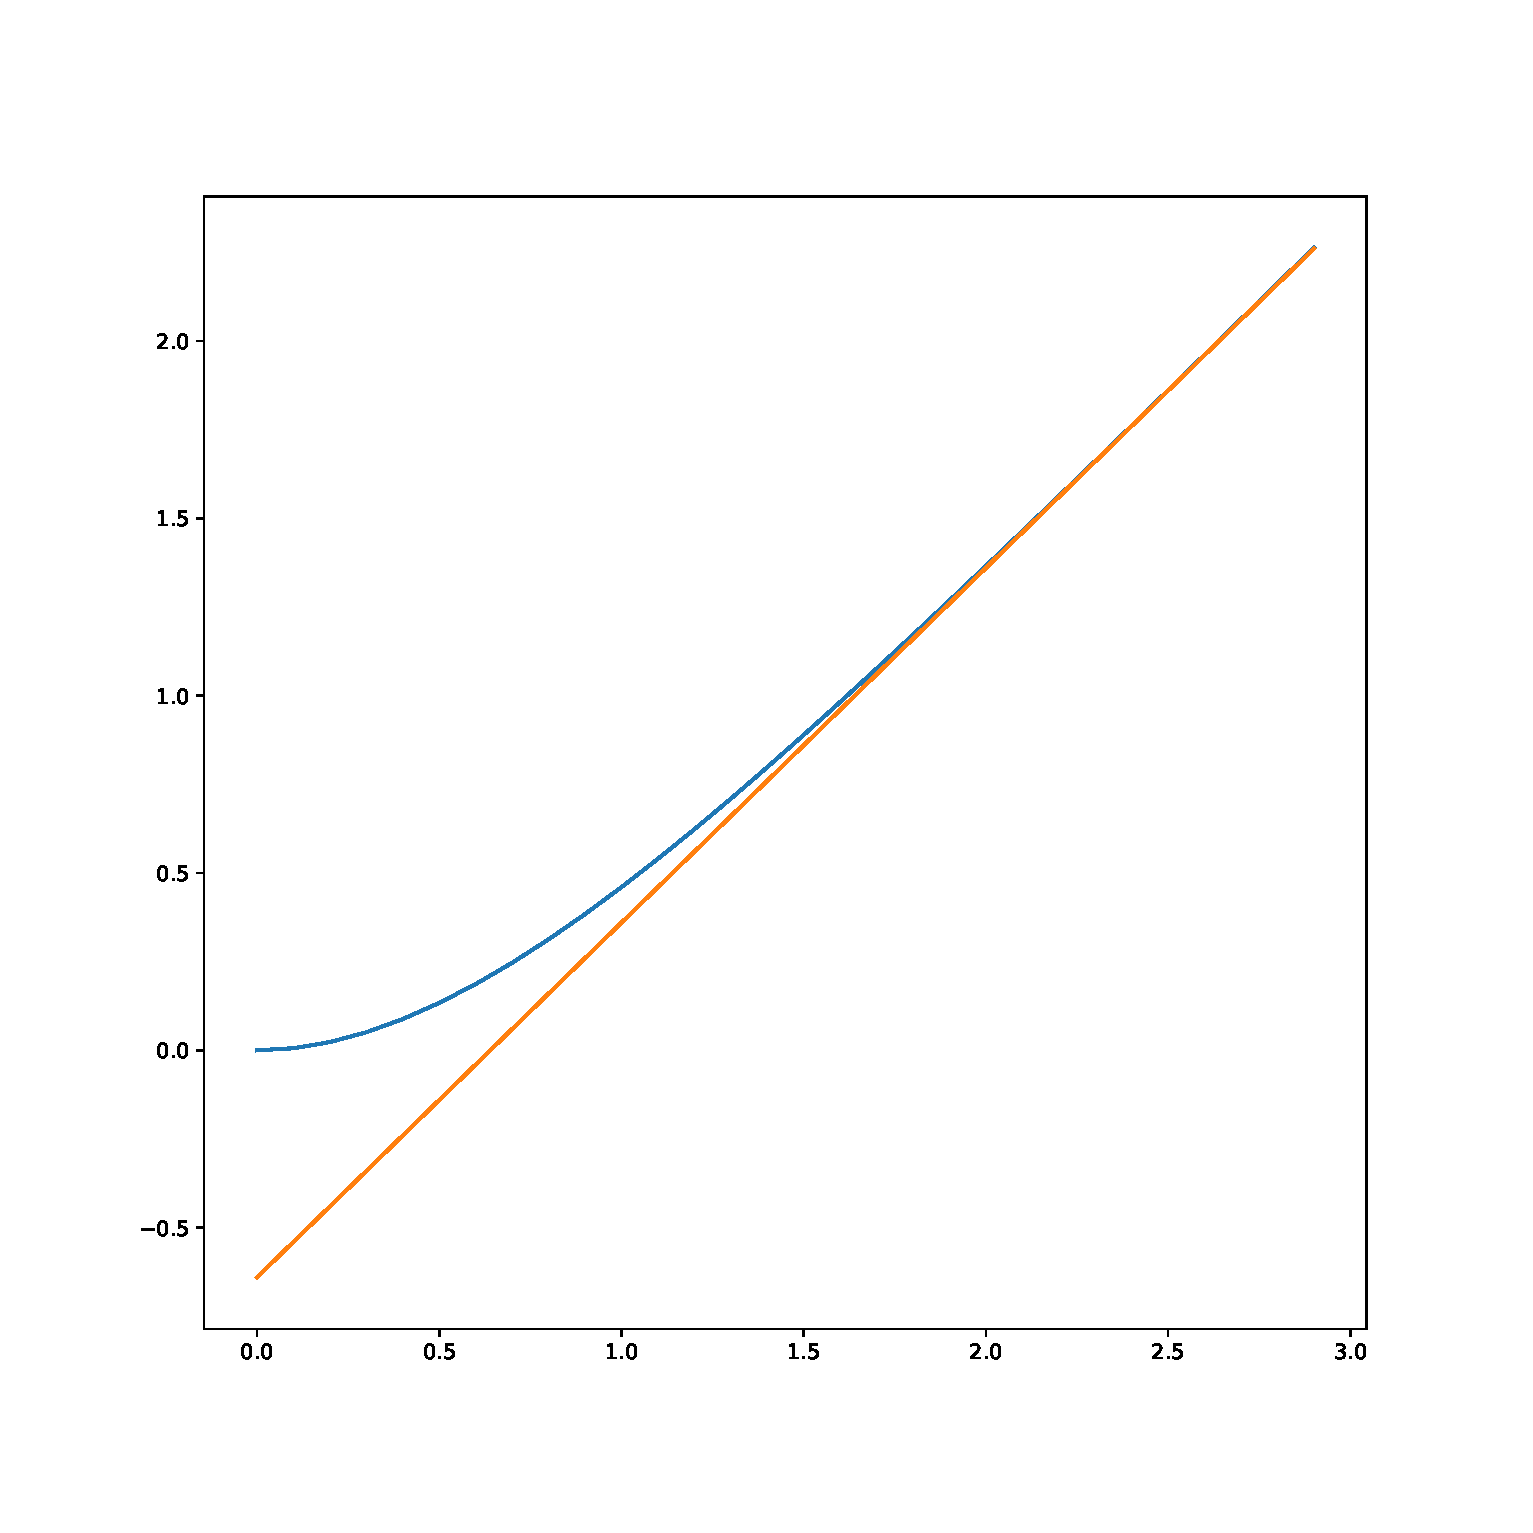
\includegraphics[width=0.4\linewidth]{figures/stagnation_function_disp}
  \caption{\label{fig:stagnation_functions}}
\end{figure}


In Figure \ref{fig:stagnation_functions} left, the function $g$ and
its first and second derivatives are plotted. With these, it is easy
to plot the resulting streamlines, Figure
\ref{fig:stagnation_streamlines} right. In the latter, the potential
streamlines are shown in the left. It is apparent how the flow is
``moved upwards'' due to viscous effects near the wall. This
displacement is readily quanfified by the asympotic behavour of $g$,
as shown in Figure \ref{fig:stagnation_functions} left. A reasonable
approximation is
\[
g(y) \approx -0.64 + y .
\]
This provides an estimate of the boundary layer thickness as given
by
\[
\delta = 0.64 \ell =  0.64 \sqrt{\nu/B} ,
\]
which then increases as the root square of $\nu$, and decreases as,
basically, the root square of the velocity far away from the wall
(through $B$).

To get some numbers, if air approaches a \SI{10}{\centi\meter}
diameter cylinder at $u_0=\SI{10}{\meter\per\second}$, then
$B = 4u_0/D =\SI{400}{\per\second}$ (there is a factor of $4$
involved, see \cite{white1991viscous} \S 7.3 ). With
$\nu\approx\SI{1.5e-5}{\meter\squared\per\second}$, we get
$\delta = \SI{0.12}{\milli\meter}$, a very thin layer. The thickness
of the layer can be defined in other ways, for example as the distance
at which $f'(y) \approx 0.99 $ (so that the value of $u_x = B x f'$ is
$99\%$ its potential solution value, $B x$.) This yields
$\approx 2.4 \ell$, which is about $3.7$ times larger than
$\delta$. Still, only approximately $ \SI{0.44}{\milli\meter}$, beyond
which the effect of the wall is quite neglibible.

This fact is a blessing, since it restores our faith in
potential-based solutions: many flows look potential flows when viewed
at some distance from obstacles (indeed, away from any region that may
generate vorticity and involve shear, such as jets, wakes \ldots). It
also solves d'Alembert's paradox, since the velocity field can still
comply with the no-slip boundary condition and exert drag forces on
obstacles (in general, they will be due both to pressure and to wall
shear stress). It is also a curse mathematically: the details of a
proper matching between it the layer and the flow around it must be
worked out carefully. Also computationally, the fact that the boundary
layer is so thin compared with other dimensions of the problem leads
to prohibitively large simulation meshes, or the necessity to refine
the meshes close to surfaces. The latter fact favours methods such as
the finite element method, or the finite volume method, in which
refinement is easier, over other ones like finite differences.

The pressure was partly known already, $p=-(B^2/2) x^2 + h(y)$. The other
Navier-Stokes equation, which we have still not used, reads
\[
B f B f'  =  - \frac{\partial p}{\partial y} -
\nu B  f'' .
\]
This means
\[
h' = - B^2 f f' - \nu B f'' ,
\]
which may be easily integrated :
\[
h = -B^2 \frac12 f^2  - \nu B f' .
\]
So, finally:
\[
p = -\frac{1}{2} \left[
  (B x)^2 +
  (B f)^2
  \right]  - \nu B f' =
 -\frac{1}{2} \left[
  (u_x / f' )^2 +
  u_y^2
  \right]  - \nu B f' ,
 \]
 where the last equality shows that the pressure is not so different
 from the potential solution, Eq. \ref{eq:p_stag_pot}.
%
 Notice it is not $u_X$ which features, but rather $u_x/f'$, which
 does tend to the $u_x$ away from the wall. An additional, viscous
 term appears, which makes the pressure have a constant offset
 $-\nu B$ with respect to its potential counterpart, as we move
 away from the wall.

 Pressures are also included in Fig.
 \ref{fig:stagnation_streamlines}. To make a more quantitative
 comparison, isobars are plotted in
 Fig. \ref{fig:stagnation_pressures}. It is interesting that viscosity
 causes pressure to be ``pushed'' against the wall, flattening the
 isobars (and, interestingly, making them not normal to the
 wall). While, far away from the wall, they approach the same circular
 shape, but with a constant offset. In these figures, pressures are
 plotted in their reduced form. It is easy to check that the pressure
 scale is given by $B \nu$ (units of velocity squared --- remember this
 is the dynamic pressure).

\begin{figure}
  \centering
  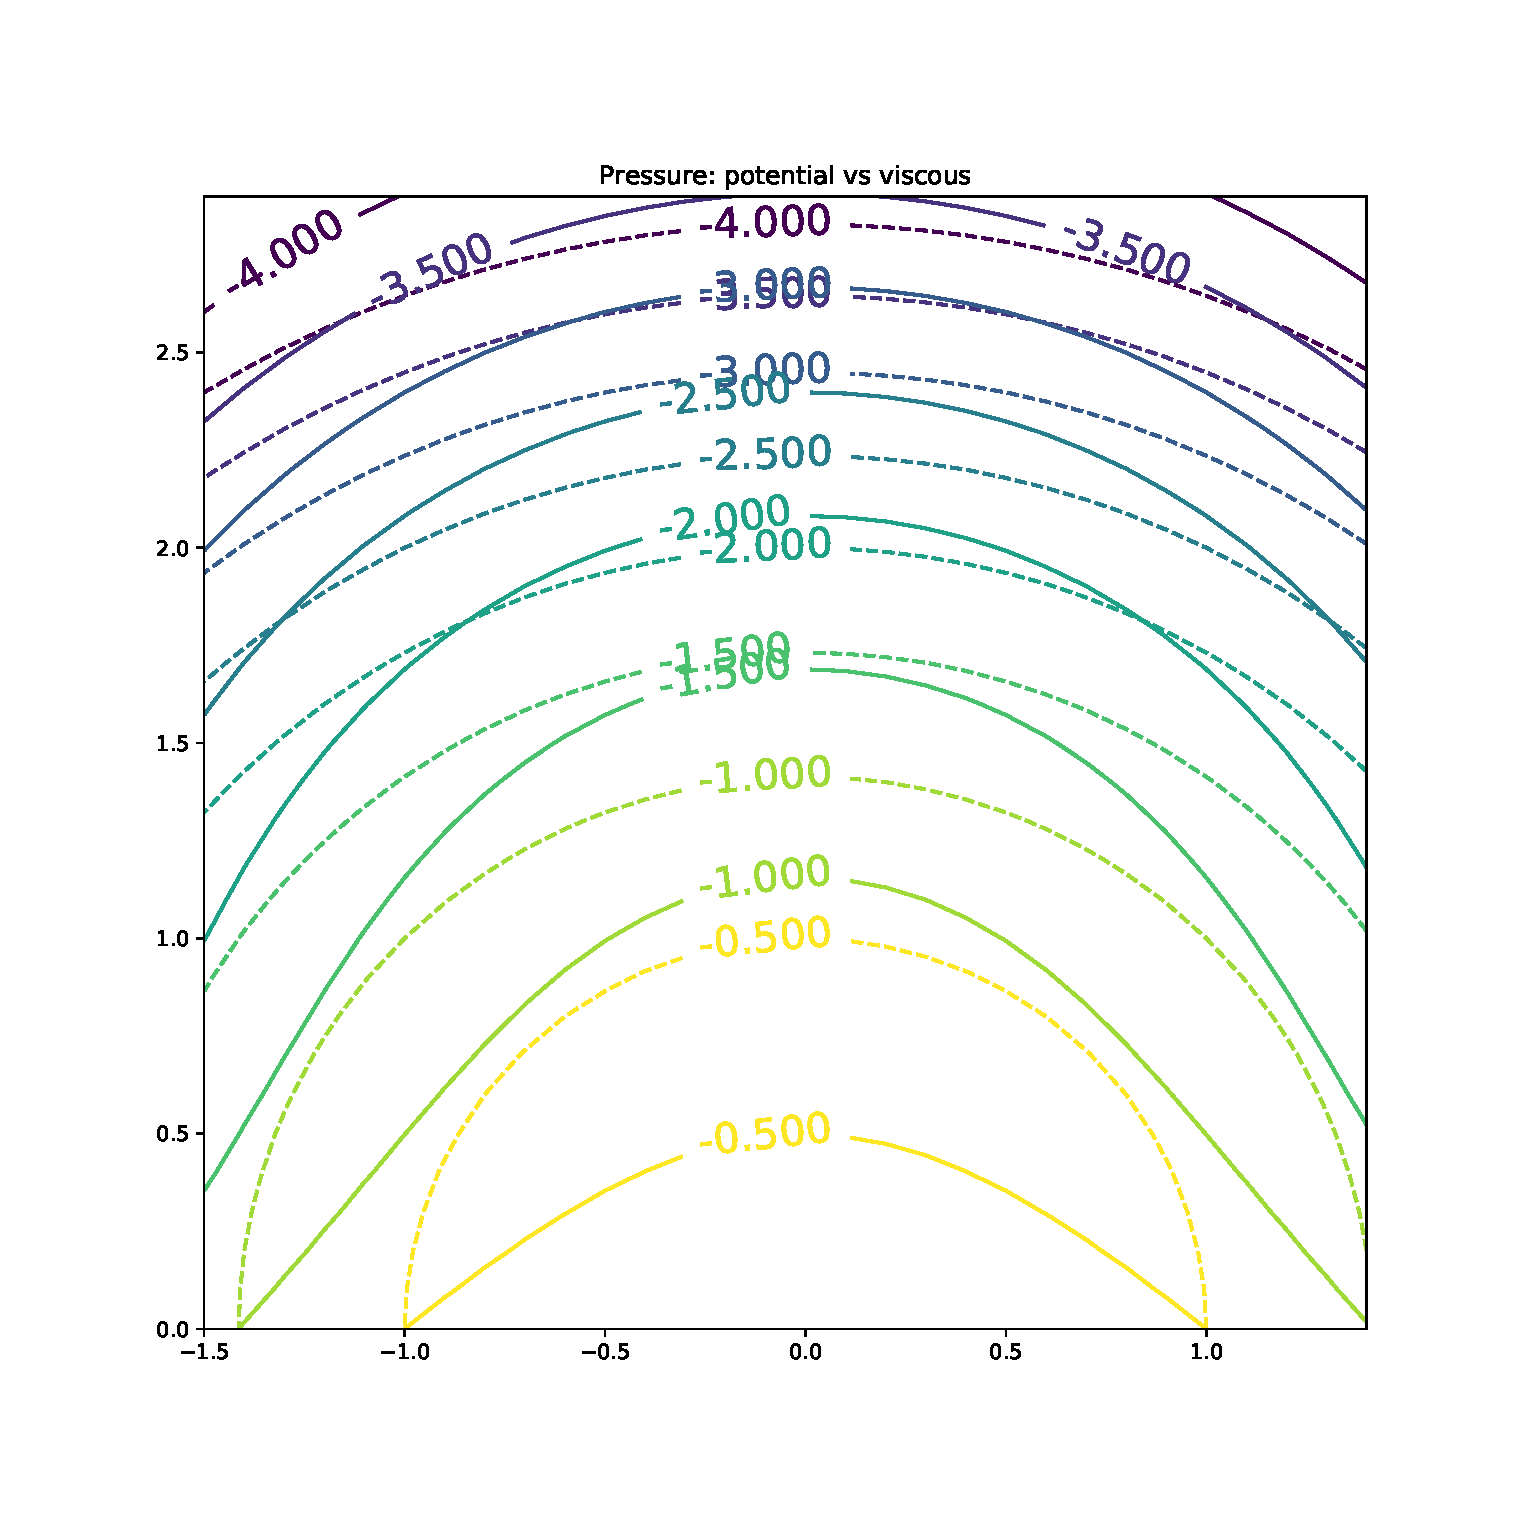
\includegraphics[width=0.6\linewidth]{figures/stagnation_potential_viscous_pressures}
  \caption{\label{fig:stagnation_pressures}}
\end{figure}

Another interesting feature of the flow is its vorticity, which is
readily computed from
\[
\omega_z =
\frac{\partial u_y}{\partial x} -
\frac{\partial u_x}{\partial y} =
0 - B x f''(y)  = - B x^* g''(y^*) .
\]
Hence the wall is seen to induce vorticity close to it, with a sign change
on both sides on the $x=0$ symmetry plane. The shear stress is given by a
similar expression,
\[
\tau_{xy}= \mu
\left(
\frac{\partial u_y}{\partial x} +
\frac{\partial u_x}{\partial y}
\right)
 =  \mu B  x f''(y)  = \mu B x^* g''(y^*) .
 \]

 In particular, the wall stress is
 \[
 \tau_\mathrm{w}:=\tau_{xy}(y=0) = \mu B x^* g''(0)
 \approx 1.234 \mu B x^*
 \]

 The (horizontal) skin friction coefficient may be defined, for this problem,
 as
 \[
 C_\mathrm{f} := \frac{2 \tau_\mathrm{w} }{ \rho (B x)^2 } .
 \]
 The denominator features the horizontal velocity away from the wall,
 $B x$. Then,
 \[
 C_\mathrm{f} := \frac{2 \sqrt{B\nu}  g''(0) }{ B x } =:
 \frac{2   g''(0) }{\sqrt{ \mathrm{Re}_x} } ,
 \]
 where the local Reynolds number is defined as
 \[
 \mathrm{Re}_x = \frac{(Bx) x}{\nu} .
 \]
 I.e. a Reynolds number where the typical velocity is the horizontal
 velocity far from the wall, $Bx$, and the distance is that to the
 impact point, $x$. A dependence of the friction coefficient with the
 inverse square root of a local Reynolds number is a common feature of
 laminar boundary layers.
 
